\documentclass[a4paper, czech]{article}

\title{Úloha č.3: Elektronkový zesilovač - Simulace}
\author{Karolína Andrea Šebestová}
\date{Datum měření: 22.10.2024}

\usepackage[czech]{babel}
\usepackage{indentfirst}
\usepackage{graphicx}
\usepackage{float}
\usepackage[margin=1.5cm]{geometry}
\usepackage{booktabs}
\usepackage{amsmath}

\begin{document}

\maketitle

\begin{figure}[H]
    \centering
    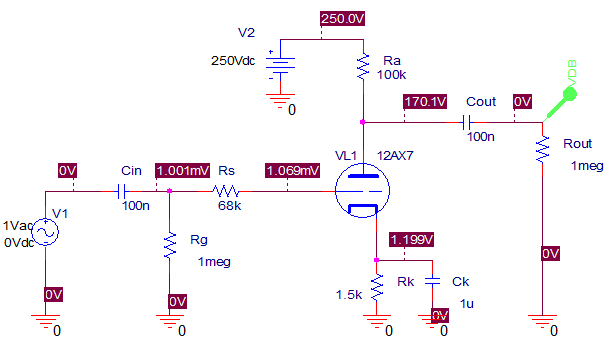
\includegraphics[width=0.5\textwidth]{schema.png}
\end{figure}

\section{Úkoly měření}

\begin{enumerate}
    \item V tomto úkolu se seznámíte s převodní charakteristikou elektronkové triody, což je závislost anodového (výstupního) proudu na (vstupním) napětí na mřížce. Otevřete projekt Prevodni char a prohlédněte si schéma. V menu PSpice, Edit Simulation Profile si prohlédněte nastavení simulace. Půjde o stejnosměrnou analýzu (DC Sweep) se změnou napětí zdroje V1 od -3 do 0 V s krokem 0,1 V. Toto nastavení neměňte (zvolte Storno) a spusťte simulaci z menu PSpice, Run (zkratková klávesa F11). V novém okně by se měla vykreslit požadovaná převodní charakteristika. Tuto charakteristiku vložte do protokolu a okomentujte ji. Zamyslete se nad vhodnou volbou pracovního bodu elektronkového zesilovače, tedy pro jaká vstupní napětí je převodní charakteristika lineární a nedojde ke zkreslení či limitaci.
    \item Nyní se budeme zabývat výstupními charakteristikami triody, tedy závislostmi výstupního proudu na napětí mezi anodou a katodou. Parametrem křivek bude napětí na mřížce. Otevřete projekt Vystupni char a prohlédněte si schéma. V menu PSpice, Edit Simulation Profile si prohlédněte nastavení simulace. Půjde opět o stejnosměrnou analýzu se změnou napětí zdroje V2 od 0 do 250 V s krokem 10 V. V tomto případě je ještě aktivována parametrická analýza (Parametric Sweep). Po kliknutí na její nastavení (vlevo v okně Options) lze vidět, že se jako parametr bude měnit napětí zdroje V1, a to od -3 do 0 V po 0,2 V. Toto nastavení opět neměňte a spusťte simulaci. Charakteristiky opět vložte do protokolu a slovně popište jejich význam.
    \item Zde bude simulována závislost přenosu (zesílení) celého zesilovače s triodou na kmitočtu. Otevřete projekt Zesilovac AC char a prohlédněte si schéma. V menu PSpice, Edit Simulation Profile si prohlédněte nastavení simulace. Je aktivována analýza AC Sweep, tedy střídavá analýza zobrazující frekvenční charakteristiky. Všimněte si rozsahu kmitočtu. Spusťte simulaci, výslednou charakteristiku vložte do protokolu a zhodnoťte ji. Změňte hodnotu Rs (např. na pětinásobek a na pětinu původní hodnoty) a zhodnoťte vliv na průběh zesílení. Podobně zjistěte také vliv změny Ck, Cin a Cout na průběh zesílení (měňte uvedené kapacity jednotlivě).
    \item V tomto úkolu budou simulovány časové průběhy signálů v obvodu. Otevřete projekt Zesilovac transient a prohlédněte si schéma. V menu PSpice, Edit Simulation Profile si prohlédněte nastavení simulace. Je aktivována analýza Time Domain (Transient), tedy časová analýza. Všimněte si parametru Run to time znamenajícího časový rozsah simulace. Spusťte simulaci, výslednou charakteristiku vložte do protokolu a zhodnoťte ji. Změňte amplitudu vstupního signálu (parametr VAMPL zdroje V1). Nastavte ji na 2 V, kdy by mělo dojít ve výstupním signálu k limitaci, což ověřte. Na základě převodní charakteristiky vysvětlete příčinu limitace jak v kladné, tak v záporné půlvlně výstupního signálu. Oba průběhy, tedy s limitací a bez, vložte do protokolu.
    \item Pomocí tlačítka FFT v okně grafických charakteristik zobrazte spektrum výstupního signálu při vstupní amplitudě 2 V. Vypočítejte harmonické zkreslení (THD - Total Harmonic Distortion) podle prvních 20-ti harmonických složek podle vztahu:
    \begin{equation*}
        THD = \sqrt{\frac{U_2^2 + U_3^2 + ... + U_{20}^2}{U_1^2 + U_2^2 + ... + U_{20}^2}} \cdot 100 \%
    \end{equation*}
    kde $U_1$ je amplituda (velikost spektrální čáry) první harmonické složky o frekvenci $f_{in}$ = 1,5 kHz, $U_2$ je amplituda následující složky o frekvenci $2 f_{in}$, $U_3$ je amplituda složky o frekvenci $3f_{in}$ atd. Při odečítání velikostí jednotlivých harmonických složek používejte kurzory a vhodně měňte měřítka os dvojklikem na osy nebo tlačítky. Zjistěte, jak bude znít zvuk s takovouto hodnotou THD.
\end{enumerate}

\section{Zpracování úkolů}

\subsection{Tabulky}

\subsection{Výpočty}

\subsection{Grafy}

\section{Závěr}

\end{document}